\documentclass{article}

%% doc settings
\hyphenchar\font=-1 % suppress hyphenation
\setlength\parindent{0pt} % suppress indentation
\usepackage[margin=1.5truein]{geometry} % set page margins

%% libraries
\usepackage{array}
\usepackage{listings}
\usepackage{fancyhdr}
\usepackage{lastpage}
\usepackage{url}
\usepackage{xcolor}
\usepackage{hyperref}
\usepackage{natbib}
\usepackage{tikz}
\usepackage{tikz-uml}
\usepackage{textcomp}

%% link appearance 
\hypersetup{
    colorlinks = true,
    linkcolor = red,
    urlcolor = red,
    citecolor = black
}

%% table & diagrams
\usetikzlibrary{
    shapes,
    arrows,
    positioning,
    calc
}

\tikzset{
    block/.style = {draw, fill=white, rectangle, minimum height=48pt, minimum width=64pt},
    round/.style = {draw, fill=white, circle},
    sum/.style= {draw, fill=white, circle, node distance=2cm},
    input/.style = {coordinate},
    output/.style= {coordinate},
}

\tikzumlset{fill usecase=white}


%% page numbers
\pagestyle{fancy}
\fancyhf{}
\fancyfoot[C]{Pg. \thepage \space of \pageref*{LastPage}}
\renewcommand{\headrulewidth}{0pt}

%% begin doc
\begin{document}
\title{SYSEN 6150: Model Based Systems Engineering\\~\\
    \Large IDEF0, Decision Matrix, GQM, AHP, CVP, Updates
}
\author{
    Nick Kunz [NetID: \url{nhk37}] \hyperlink{nhk37@cornell.edu}{nhk37@cornell.edu}
}
\date{October 7, 2022}
\maketitle
\thispagestyle{fancy}

%% body
\section*{IDEF0}
The following diagram exhibits a subset of the broader system of data collection and pre-processing, beginning at the API level and truncated at data parsing and object mapping.

\\~\\
\\~\\

%% drawing
\begin{center}
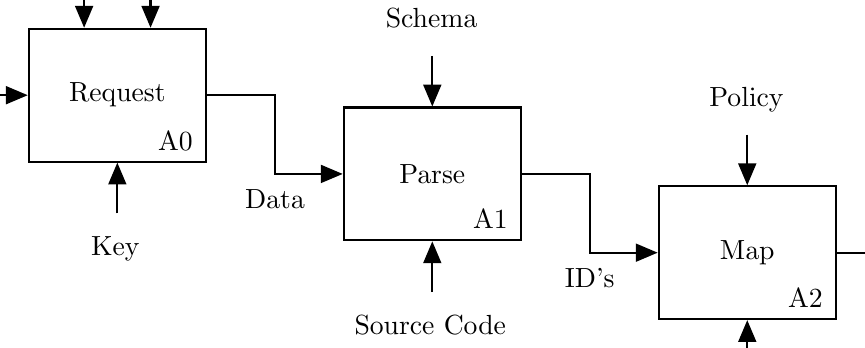
\begin{tikzpicture}[auto, thick, >=triangle 45]

    %% nodes
    \draw node at (-1, 0) [input, name = server]{};
    \draw node at (1, 1.5) [input, name = rate]{};
    \draw node at (1, -1.5) [input, name = key]{};
    \draw node at (1, 0) [block, name = request, label={[xshift=21pt, yshift=-48pt]A0}]{Request};

    \draw node at (5, 0.5) [input, name = schema]{};
    \draw node at (5, -2.5) [input, name = source]{};
    \draw node at (5, -1) [block, name = parse, label={[xshift=21pt, yshift=-48pt]A1}]{Parse};

    \draw node at (9, -0.5) [input, name = sort]{};
    \draw node at (11, -2) [input, name = entities]{};
    \draw node at (9, -3.5) [input, name = object]{};
    \draw node at (9, -2) [block, name = map, label={[xshift=21pt, yshift=-48pt]A2}]{Map};

    %% edges
    \begin{scope}[transform canvas={xshift=0pt}]
        \draw[->] (server) -- node [xshift=-12pt, yshift=-3pt, label=left:Server]{}(request);
    \end{scope}
    
    \begin{scope}[transform canvas={xshift=12pt}]
        \draw[->] (rate) -- node [xshift=-4pt, yshift=12pt, label=above:Rate]{}(request);
    \end{scope}

    \begin{scope}[transform canvas={xshift=-12pt}]
        \draw[->] (rate) -- node [xshift=-4pt, yshift=12pt, label=above:Size]{}(request);
    \end{scope}

    \begin{scope}[transform canvas={xshift=0pt}]
        \draw[->] (key) -- node [xshift=3pt, yshift=-10pt, label=below:Key]{}(request);
    \end{scope}

    \begin{scope}[transform canvas={yshift=0pt}]
        \draw[->] (request) -- +(2, 0) |- node [xshift=0pt, yshift=-2pt, label=below:Data]{} (parse);
    \end{scope}

    \begin{scope}[transform canvas={xshift=0pt}]
        \draw[->] (schema) -- node [xshift=-4pt, yshift=12pt, label=above:Schema]{}(parse);
    \end{scope}    

    \begin{scope}[transform canvas={xshift=0pt}]
        \draw[->] (source) -- node [xshift=3pt, yshift=-10pt, label=below:Source Code]{}(parse);
    \end{scope}

    \begin{scope}[transform canvas={yshift=0pt}]
        \draw[->] (parse) -- +(2, 0) |- node [xshift=0pt, yshift=-2pt, label=below:ID's]{} (map);
    \end{scope}

    \begin{scope}[transform canvas={yshift=0pt}]
        \draw[->] (sort) -- node [xshift=-4pt, yshift=10pt, label=above:Policy]{}(map);
    \end{scope}
    
    \begin{scope}[transform canvas={yshift=0pt}]
        \draw[->] (map) -- node [xshift=16pt, yshift=-4pt, label=right:Entities]{} (entities);
    \end{scope}

    \begin{scope}[transform canvas={xshift=0pt}]
        \draw[->] (object) -- node [xshift=3pt, yshift=-11pt, label=below:Object Dictionaries]{}(map);
    \end{scope}
    
\end{tikzpicture}
\end{center}

\newpage
\section*{Decision Matrix}

The following diagram exhibits 3 measures of effectiveness given its attributes.\\

    \begin{tabular}{ | m{80pt} | m{28pt}| m{28pt} | m{28pt} | m{28pt} | m{36pt} | m{28pt}| m{28pt} | m{28pt} | }
        \hline
        \multicolumn{1}{|l|}{\space} & \multicolumn{3}{|l|}{Normal Score} & \multicolumn{2}{|l|}{User Depend.} & \multicolumn{3}{|l|}{Final Score} \\
        \hline    
        \textbf{Criteria} & \textbf{A} & \textbf{B} & \textbf{C} & \textbf{Score} & \textbf{Weight} & \textbf{A} & \textbf{B} & \textbf{C} \\ 
        \hline
        Latency & 5 & 5 & 5 & 5 & 3 & 15 & 15 & 15 \\ 
        \hline
        Asymptotics & 4 & 5 & 6 & 3 & 4 & 16 & 20 & 24 \\ 
        \hline
        Accuracy & 10 & 10 & 10 & 7 & 5 & 50 & 50 & 50 \\ 
        \hline
    \end{tabular}

\section*{Goal Question Metric (GQM)}

The following diagram exhibits the goals of the system and how they might be measured.\\

    \begin{tabular}{ | m{56pt} | m{96pt}| m{72pt} | m{70pt} | m{68pt} | }    
        \hline
        \textbf{Goal} & \textbf{Question} & \textbf{Ideal Metric} & \textbf{Appx. Metric} & \textbf{Data Collect.}\\ 
        \hline
        Make system fast. & How long do requests take to complete? & Wall clock time. & Asymptotic complexity. & Service logging.\\ 
        \hline
        Make system reliable. & What is the estimated downtime? & Ratio of time without service. & User reported bugs & Service logging.\\ 
        \hline
        Make system inform. & Does it respond with actionable insights? & Reported real world actions. & User engagement. & Service logging.\\ 
        \hline
        Make system improve. & Are there software updates? & Software releases. & Code commits and PR's. & Git history and DevOps.\\ 
        \hline
        Make system local. & Can it work both online and offline? & Offline testing pass. & (No substitute) & Service logging.\\ 
        \hline
    \end{tabular}

\section*{Analytical Hierarchy Process (AHP)}

The following diagram exhibits the system requirements in different contexts and perspectives.\\

    \begin{tabular}{ | m{32pt} | m{32pt} | m{32pt} | m{32pt} | m{32pt} | m{32pt} | m{32pt} | m{32pt} | m{32pt} | }
        \hline
        \multicolumn{2}{|l|}{Make system fast.} & \multicolumn{3}{|l|}{Make system reliable.} & \multicolumn{2}{|l|}{Make system inform.} & \multicolumn{2}{|l|}{Make system local.} \\
        \hline
        \multirow{\rotatebox{90}{Make the system fast for users. }} & \multirow{\rotatebox{90}{Make the system fast for systems. }} & \multirow{\rotatebox{90}{Make the system reliable for users. }} & \multirow{\rotatebox{90}{Make the system reliable for devs.}} & \multirow{\rotatebox{90}{Make the system reliable for systems.}} & \multirow{\rotatebox{90}{Make the system drive user decisions.}} & \multirow{\rotatebox{90}{Make the system drive dev decisions.}} & \multirow{\rotatebox{90}{Make the system work offline for users.}} & \multirow{\rotatebox{90}{Make the system work offline for systems. }} \\
        \hline

    \end{tabular}

\newpage
\section*{Customer Value Proposition (CVP)}
Real-time analysis of urban phenomena is an important field of research to address the growing demand for low-latency time-dependent decision making. In order to provide this information to both end-users and analyst, the proposed system introduces a fast, reliable, and informative application service to explore the environmental effects of transit systems.\\

Directly addressing the need for low-latency data, an application service has been developed to handle a typical response time of 1 sec. on 1 min. intervals of vehicle idling. There is no known system that allows for these real-time calculations and those that have addressed it in the literature, do not maintain a production system for public use. \\

The system has also been designed for fault tolerance, where multiple requests are made before time out or termination in the event that the service is not online. This feature addresses the practical need for data persistence over varying time-scales in the event that the system or one of its components (mainly physical data collection) is unavailable.\\

The system provides useful information meant for direct user consumption or for future analyses. It is important that the data produced from the system is available at a rate where intra-hour spatio-temporal analyses can be conducted at a locally meaningful geographic resolution of less than 0.25mi of accuracy. 

\\~\\

\section*{Updates}
In the previously exhibited IDEF0 diagram, the \textit{``Request''} action is currently completed. The \textit{``Parser''} action is near completion as of October 7th, 2022. The \textit{``Map''} action is currently under development. The scope beyond what was exhibited in the IDEF0 diagram is scheduled for development in November, 2022. Analyses will begin December, 2022. 

\end{document}